\chapter{A Language for Metamodelling}
\label{xmofchapter}

\section{Introduction}

As we saw in the previous chapter, a metamodel should not only be
able to describe the modelling concepts provided by the language
(its abstract syntax), but also many other important features of a
language definition, including semantics  (the meaning of the
language), concrete syntax (how the language is presented) and
other features such as relationship to other languages in the world
around it.

Any metamodelling language appropriate for describing languages
must be expressive enough to capture all these different aspects in
a platform independent way. In other words, the resulting
metamodels should be self sufficient and independent of
implementation specific descriptions of the language being
modelled. Thus, reliance on the implementation of the language's
behaviour in an external programming language, or the assumption
that there will be an external database which manages object
creation and persistence should be completely avoided.

The language presented in this chapter does just this. This
language, which we call XMOF, combines and extends a number of
standard modelling facilities to provide a minimal, but expressive,
platform independent language for metamodelling. XMOF includes the
following features:

\begin{itemize}

\item Support for standard OO modelling concepts such as packages, classes, and
associations to describe language concepts and their relationship to one another.

\item A constraint language, which can used to describe well-formedness rules.

\item A set of action primitives, which can be used to capture the behavioural semantics of a language.

\item A language for expressing mappings between languages and language components.

\item A concrete syntax language which can be extended to support new concrete syntaxes of languages with ease.

\item A generic metamodel framework, which supports standard plug-points and machinery for
expressing model element instantiation, execution, expression evaluation and reflection.

\end{itemize}

\section{XMOF Features}

The following sections present an overview of the key features of
XMOF. This is not a full definition, but will reference fuller
descriptions of the components of the language where appropriate.

\subsection{OO modelling concepts}

XMOF provides the standard OO modelling concepts that are supported
by MOF and UML, including packages, classes and associations.
Traditionally, these are  visualised using class diagrams. Figure
\ref{classDiagram} shows an example of a class diagram of a simple
model consisting of a package with a number of classes and
associations. This model describes a simple state machine, where a
state machine contains states and transitions, and transitions have
source and target states.

\begin{figure}[htb]
\begin{center}
\includegraphics[width=8cm]{XMOF/figures/classDiagramExample}
\caption{An example of a class diagram}
\label{classDiagram}
\end{center}
\end{figure}

XMOF also provides a concrete syntax for packages and classes. The
equivalent concrete representation of the state machine class
diagram shown in figure \ref{classDiagram} is shown below.

\small
\begin{verbatim}
1 @Package StateMachine
2    @Class isAbstract Named
3      @Attribute name : String end
4    end
5    @Class StateMachine
6      @Attribute states : Set(State) end
7      @Attribute transitions : Set(Transition) end
8      @Attribute startingState : State end
9    end
10    @Class State extends Named
11   end
12   @Class Transition extends Named
13     @Attribute source : State end
14     @Attribute target : State end
15   end
16 end
\end{verbatim}

Here, line 1 shows the start of a package named StateMachine, which
contains all the sub-definitions relating to state machines.

Line 2 contains the start of a class definition for the class
Named,  which is an abstract class for a named element. Line 5 is
the start of the definition of the StateMachine class. It defines
two attributes named states and transitions, whose types are
Set(State) and Set(Transition). These types correspond to the "*"
multiplicity of the equivalent association ends in the class
diagram.

Lines 10 and 12 are the start of the State and Transition class
definitions. Both these classes specialise the class Named, and
therefore inherit a name attribute. A Transition has two attributes
source and target, which are of type State. The fact that they are
single valued reflects the multiplicity of the equivalent
association ends in the class diagram.

As chapter \ref{concretesyntax} will show, the concrete
representation  of a modelling language should be clearly
distinguished from its abstract syntax representation. Here, two
different concrete syntaxes are essential being used to capture the
same information.

\normalsize

\subsection{Constraints}

It is often necessary to make well-formedness statements about
concepts in a model.  These statements are often made informally,
for example in the context of figure \ref{classDiagram} it might be
useful to specify that \emph{all transitions have unique names
within a state machine}. A constraint language provides a means of
succinctly expressing complex well-formedness rules unambigiously.
For example the well-formedness statement mentioned above can be
added to the class StateMachine in the following way:

\small
\begin{verbatim}
context StateMachine::StateMachine
  @Constraint NoTwoTransitionsWithTheSameName
    self.transitions->forAll(t1 |
      self.transition->forAll(t2 |
        t1.name = t2.name implies t1 = t2))
  end
\end{verbatim}
\normalsize

Another well-formedness rule requires that the starting state must
be one of the states of the state machine:

\small
\begin{verbatim}
context StateMachine::StateMachine
  @Constraint ValidStartingState
    not self.states->isEmpty implies self.states->includes(self.startingState)
  end
\end{verbatim}
\normalsize

The constraint language used in XMOF is OCL. The primary
difference between the OCL used here and the standard OCL language
is in the use of a different syntax for declarations. In this case
''@Constraint'' is used as opposed to the ''inv:'' declaration used
in standard OCL. The reasons for this choice will become apparent
later when we consider the need for a flexible parsing language.

\subsection{Queries}

OCL can be used to write queries. A query is used to produce a
value in the context of a current object state; it does not cause
any side effects. The following is an example of a query:

\small
\begin{verbatim}
@Class StateMachine
  @Operation getState(n:String):State
    self.states->select(s | s.name = n)->sel
  end
end
\end{verbatim}
\normalsize

This will filter the states of a state machine, selecting those
states whose name matches the string n. Here, sel, is an inbuilt
operation, which selects a single element from a collection. This
is required in order to return a single State. sAgain, note that
the declaration of a query diffes from that in the OCL standard.

\noindent Another example of query returns true if there exists a
state with the name, n:

\small
\begin{verbatim}
@Class StateMachine
  @Operation isState(n:String):Boolean
    self.states->exists(s | s.name = n)
  end
end
\end{verbatim}
\normalsize

\subsection{Actions and XOCL}

OCL is by design a static language and does not change the state of
objects it refers to.  In some situations this is a good thing
because it guarantees side-effect free evaluation.  However this
limitation makes it very difficiult to describe operational
behaviour in a way which can be readily executed.  Standard OCL
does provide pre-/post- conditions as a way of specifying the
effect of an operation, however, in general these cannot be
executed.

A more useful approach is to augment OCL with action primitives.
The XOCL language extends OCL with a number of key behaviour
primitives, as chapter \ref{} demonstrates, this is a essential
step towards making XMOF a true meta-programming environment.

An example of the application of actions in XOCL can be seen in
the state machine of figure \ref{classDiagram}. If it was
requirement to be able to add new states to the state machine
dynamically then the following XOCL statement can be written:

\small
\begin{verbatim}
context StateMachine
  @Operation addState(name:String)
    self.states := self.states->including(State(name))
  end
end
\end{verbatim}
\normalsize

New instances of classes can be created by declaring the class as
an operation. In this example a new instance of a State is created
by the declaration \emph{State()}. The resulting object is then
assigned to the set of states that includes the new state using the
assignment expression \emph{:=}. It is important to recognise that
\emph{:=} and \emph{new} have an imperative semantics and (given an
appropriate implementation) can be executed.

In the above example, the State() operation takes initialisation
value, which is the name of the state that is to be created. To
handle initialisation parameters, a special operation called init()
is provided. It takes a sequence of values as an argument, which
are then used to intialise the object's slots. In the case of the
state machine, three such operations are required, one for each
concrete class. The first intialises the name of a state, the
second assigns a name, and a source and target state to a
transition, and the third initialises a new state machine with a
starting state, set of transitions, and set of states:

\small
\begin{verbatim}
context State
  @Operation init(args)
    self.name := args->at(0)
  end
end

context Transition
  @Operation init(args)
     self.name := args->at(0);
     self.source := args->at(1);
     self.target := args->at(2)
  end

context StateMachine
  @Operation init(args)
     self.startingState := args->at(0);
     self.states := args->at(1);
     self.transitions := args->at(2)
  end
\end{verbatim}
\normalsize

The body of the next example illustrates how OCL conditional
expressions and logical operators can be combined with XOCL actions
to define the operation of adding a transition. This operation
takes the name the new transition and the name of a source and
target state. The isState() query is then used to check that the
states belong to the statemachine before creating a transition
between them. The last line of the if statement shows how XOCL
deals with the printing of strings to the terminal.

\small
\begin{verbatim}
context StateMachine
@Operation addTransition(name:String,source:String,target:String)
  let s = State(source);
      t = State(target) in
    if self.isState("source") and self.isState("target") then
      self.transitions := self.transitions->including(Transition(name,s,t))
    else
      "Invalid State in addTransition()".println()
    end
  end
end
\end{verbatim}
\normalsize

As this example show, augmenting OCL with a small number of action
primitives results in a powerful and expressive programming
language. Furthermore, as we will see in later chapters of this
book, because the language works at the XMOF level, it also
provides a rich meta-programming environment that can be used to
construct powerful modelling facilities such as model simulators,
execution engines and compilers. Indeed, it is sufficiently
expressive to enable a complete definition of all the languages in
this book to be constructed.

\subsection{Snapshots}

A useful notation for visually representing the instances of a
metamodel is a snapshot - a notation popularised by the Catalysis
method \cite{Catalysi}. A snapshot shows objects, the values of
their slots (instances of attributes) and links (instances of
associations). A snapshot of a metamodel will thus show objects and
links that are instances of elements in the metamodel. The example
shown in figure \ref{snapshotExample} is a snapshot of the
statemachibe metamodel, and shows an instance of a statemachine
containing three states and two transitions.

\begin{figure}[htb]
\begin{center}
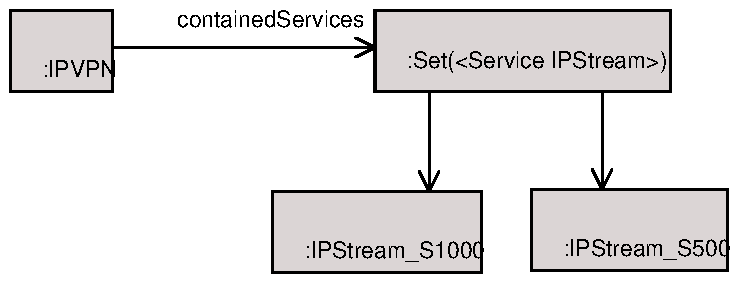
\includegraphics[width=8cm]{XMOF/figures/snapshot.pdf}
\caption{A snapshot showing an instance of the statemachine metamodel}
\label{snapshotExample}
\end{center}
\end{figure}

\subsection{Mappings}

Chapter \ref{} highlighted the fact that many languages are used
to design systems from a multitude of perspectives.  There must
exist relationships between the perspectives in order to understand
what one model means in terms of another.  These relationships are
implemented by a mapping language which specifies how we can
translate one language into another.  The mapping language used,
XMap, is a declarative, but executable language based on pattern
matching. Whilst this language can be viewed as a XMOF plug-in (as
opposed to a core part of the XMOF language), it is nevertheless
important for its ability express mappings in an intuitive, yet
ultimately implementable way.

To illustrate the use of XMap, figure \ref{cppExample} shows a
simple model of {C++} classes which will be used as the target of a
mapping from a state machine.

\begin{figure}[htb]
\begin{center}
\includegraphics[width=8cm]{XMOF/figures/cppExample}
\caption{A simple model of C++ classes}
\label{cppExample}
\end{center}
\end{figure}

A {C++} class is a namespace for its attributes and operations
(methods). An attribute has a type, and for the purposes of this
example, its type may either be another class or an enumeration
type. An enumeration type has a value, which is the sequence of
strings in the enumeration. An operation has a name and a body,
which contains a simple string representation of the body of the
operation.

A mapping from from the state machine model in figure
\ref{classDiagram}  to the {C++} in \ref{cppExample} can be
defined. This maps a state machine to a {C++} class, where each
state in the state machine is mapped to a value in an enumerated
type called STATE. Eeach transition in the state machine is mapped
to a {C++} operation with the same name and a body, which changes
the state attribute to the target of the transition.

The mapping can be modelled in XMap as shown in figure
\ref{mapping}.  The arrows represent mappings between elements of
the two languages. The first mapping, SM2Class, maps a state
machine to a C++ class. The second mapping, Transition2Op, maps a
transition to an operation.

\begin{figure}[htb]
\begin{center}
\includegraphics[width=8cm]{XMOF/figures/cppMapping}
\caption{A mapping between state machines and C++ classes}
\label{mapping}
\end{center}
\end{figure}

In order to describe the details of the mapping, XMap uses a
textual  mapping language based on pattern matching. Working
backwards, the definition of the mapping between a transition and
an operation is as follows:

\small
\begin{verbatim}
@Map Transition2Op
  @Clause Anonymous
    @Object(StateMachine::Transition,t)
      @Slot name = N end
    end
    when true
    do
    @Object(CPP::Operation)
      @Slot name = N end
      @Slot body = B end
    end
    where
      B = "state := " + self.target.name
  end
end
\end{verbatim}
\normalsize

A mapping consists of a collection of clauses, which are pattern
matches between source and target objects. Whenever a source object
is successfully matched to the input of the mapping, the resulting
object in the do expression is generated. Variables can be used
within clauses, and matched against values of slots in objects.
Because XMap builds on XOCL, XOCL expressions can also be used to
capture complex relationships between variables.

In this example, whenever the mapping is given a Transition with a
name equal to the variable N, it will generate an instance of the
class Operation, whose name is equal to N and whose body is equal
to the variable B. The where clause is used to define values of
variables, and it is used here to define the variable B to be
concatanation of the text "state := " with the target state name.
For instance, given a transition between the states "On" and "Off",
the resulting operation will have the body "state := Off". Note
that it would be quite possible to model a part of the syntax of
{C++} expressions, and equate B with an instance of an expression.

The mapping between state machines and {C++} classes is shown below:

\small
\begin{verbatim}
 @Map SM2Class
   @Clause Anonymous
     @Object(StateMachine::StateMachine)
       @Slot states = S end
       @Slot transitions = TS end
     end
     when true
     do
     @Object(CPP::CPPClass)
       @Slot attributes =
         Set{@Object(CPP::CPPAtt)
           @Slot name = "state" end
           @Slot type = T end
         end}
       end
       @Slot operations = O end
     end
     where
       T = @Object(CPP::EnumerationType)
         @Slot name = "STATE" end
         @Slot value = S->iterate(s Q=Seq{} | Q + s.name)
       end
       end;
       O = TS->collect(t | (Transition2Op.new())(t))
    end
  end
end
\end{verbatim}
\normalsize

Here, a state machine with a set of states, S, and a set of
transitions, TS, is mapped to a {C++} class with a distinguised
attribute "state" of type T, and a set of operations, O. The value
of T is an EnumerationType whose name is "STATE" and whose values
are the names of the states in S. Finally, the transitions are
mapped to operations by iterating through the transitions in TS and
applying the Transition2Op mapping.

This mapping illustrates the power of the XMap language in being
able to match arbritrarily complex structures of source and target
objects. For example, as shown by the CPPClass, source and target
objects may be nested within objects to any depth, whilst complex
rules for determining the values of slots in objects can be readily
constructed in OCL.

\subsection{Concrete Syntax}

The concrete syntax of a modelling language defines the notation
that is used to present models in the language. A notation may be
textual, or diagrammatical, or a mxuture of both. A key part of any
metamodelling language is the ability to model both these aspects,
and as a result facilitate the rapid creation of parsers and
diagram editors for a new language.

\subsection{Textual Syntax}

XMOF provides a generic parser language that can be used to model
the textual syntax of any language. This language, called XBNF (the
reader will be starting to see a pattern to our naming conventions
by now!) allows new textual constructs to be defined that can be
used as input to a model parser.

\noindent These new constructs to be defined as:

\small
\begin{verbatim}
@<NAME>
  <BODY>
end
\end{verbatim}
\normalsize

\noindent where <NAME> is the name of the construct and <BODY> is
an XBNF expression.

An XBNF expression consists of a number of BNF definition within
which XOCL variables are embedded, followed by an XOCL expression.
When a construct is parsed, the XBNF expression is used to match
each parsed element with the variables. These variables can then be
used within the XOCL action to create instances of classes that
populate a language metamodel.

Imagine that we wish to create a concrete syntax for the simple
state machine example. One part of this task would be to create a
concrete syntax for states. This might take the form:

\small
\begin{verbatim}
@State On
end
@State Off
end
\end{verbatim}
\normalsize

The following XBNF defines the syntax for parsing states and
populating instances of the class State.

\small
\begin{verbatim}
State ::= 'state' '(' name = Name ')' {State(name)}
\end{verbatim}
\normalsize

\noindent Now we have a new construct. When we type:

\small
\begin{verbatim}
  @State X end
\end{verbatim}
\normalsize

\noindent we will get:

\small
\begin{verbatim}
<State X> returned.
\end{verbatim}
\normalsize

\section{XMOF Metamodel}

As outlined in the previous chapter, XMOF follows the golden braid
metamodel architecture, and therefore is metamodelled in its own
language. Understanding the architecture of this metamodel is
important for many reasons. Firstly, the architecture is a good
example of an XMOF metamodel definition in its own right - the fact
that the XMOF metamodel is both self describing and self supporting
makes a strong statement about the expressibility of the language.
Secondly, the XMOF metamodel acts as a root for many other
metamodel definitions. For instance, it can be viewed as a subset
of the UML metamodel, and many other types of modelling languages
can also be viewed as extensions of the core architecture.

Figure \ref{xmofOverview} shows the key components of the XMOF
metamodel. The classes and relationships in the metamodel
correspond precisely to the modelling features that have been used
in this chapter to model the abstract syntax, semantics and
concrete syntax of the statemachine language. For example, the
package and classes shown in the state machine abstract syntax
metamodel in figure \ref{classDiagram} can be viewed as concrete
syntax representations of instances of the classes XMOF::Package
and XMOF::Package. The concrete syntax model can be viewed as a
representation of an instance of the class Grammar, and so on.

\begin{figure}[htb]
\begin{center}
\includegraphics[height=17cm]{XMOF/figures/XMOFSimple.pdf}
\caption{Overview of XMOF Architecture}
\label{xmofOverview}
\end{center}
\end{figure}

As we discuss the modelling of abstract syntax and semantics in
more detail in later chapters, many of the features of the
metamodel will become more understandable. There are however, some
key features that it is useful to point out here.

\begin{description}
\item[Elements and Objects] The most fundemental modelling concepts in XMOF are
elements and objects. Elements are the root of all modelling concepts, in other
words, every type of modelling concept in XMOF is an element. Elements do not
have structure or state. Objects on the hand are elements that encapsulate data
values - called slots in XMOF. An object's slots must conform to the name and
type of the attributes of the class it is an instance of.
\item[Performable] The performable class represents the root of all modellng
concepts that can be evaluated in the context of an environment (a collection
of variable bindings) to return a result. An OCL expression is a good example
of a performable concept.
\item[Classification] In XMOF, some types of modelling elements
are modelled as Classifiers. A Classifier is an element that can be
instantiated via the new() operation to create new instances. Good
examples of these elements are classes and datatypes, which can be
instantiated to create objects and datavalues. All elements have an
of() operation, which returns the classifier that the element was
instantiated from. So for example, the objects statemachine1, statemachine2
will return the class StateMachine, whilst the object fido, might return
the class Dog.
\item[Reflection]
An important property of all XMOF models is that classifiers are also objects.
This apparently strange assumption means that effectively classes and datatypes
can also be viewed as being instances of classifiers. In this case, they will
be instances of the classes XMOF::Class and XMOF::DataType. This capability
is an important one, as it enables any operation that can be carried out on
an object such as executing its operations, or mapping it to another object
can also be applied to elements at the XMOF level.
\item[XOCL] The XOCL class is an extension of OCL, and is the root of all
imperative expressions that can change the state of a model (not shown here).
\item[Snapshot] A snapshot is a collection of elements, and may therefore
include any type of element that is availble in XMOF.
\item[Grammar] A grammar can be evaluated in the context of sequence of
tokens to generate an instance of a model.
\end{description}

\section{Extensions to support reuse}

Metamodels can often be complex and time consuming to construct.
Because  the metamodelling languages is OO then some support for
reuse of metamodels is provided using class specialisation.  The
problem with this type of reuse in the context of metamodels is
that it is too fine grained.  Metamodels often share architectural
patterns, the components of which are distributed across many
classes.  It is these architectural patterns that need to be reused
rather than their components.  One solution to this is a coarse
grained reuse mechanism called templates which is also included in
UML 2.0.  Templates enable patterns to be encapsulated into
reusable units that can subsequently be used to define metamodels.
XMOF utilises templates as one of its key reuse mechanisms.

Figure \ref{templateExample} shows an example of the application to
templates to the class diagram of figure \ref{classDiagram}.  In
this the \emph{Namespace} template describes a pattern where a
\emph{Namespace} owns a number of \emph{NamedElement}.  The OCL
constraint augments this definition by specifying that each of the
named elements must have a distinct name.  A concrete metamodel is
derived from templates by passing parameters into one or more
templates.  In the case of figure \ref{templateExample},
\emph{Namespace} is substituted for \emph{StateMachine} and
\emph{NamedElement} for \emph{State} in one instantiation of the
template, and \emph{Namespace} is substituted for
\emph{StateMachine} and \emph{NamedElement} for \emph{Transition}
in a further instantiation.  The resulting definition is merged,
but more details of that will be given in chapter \ref{}.  The
important point is that the resulting metamodel is
indistinguishable from the one shown in figure \ref{classDiagram}.

\begin{figure}[htb]
\begin{center}
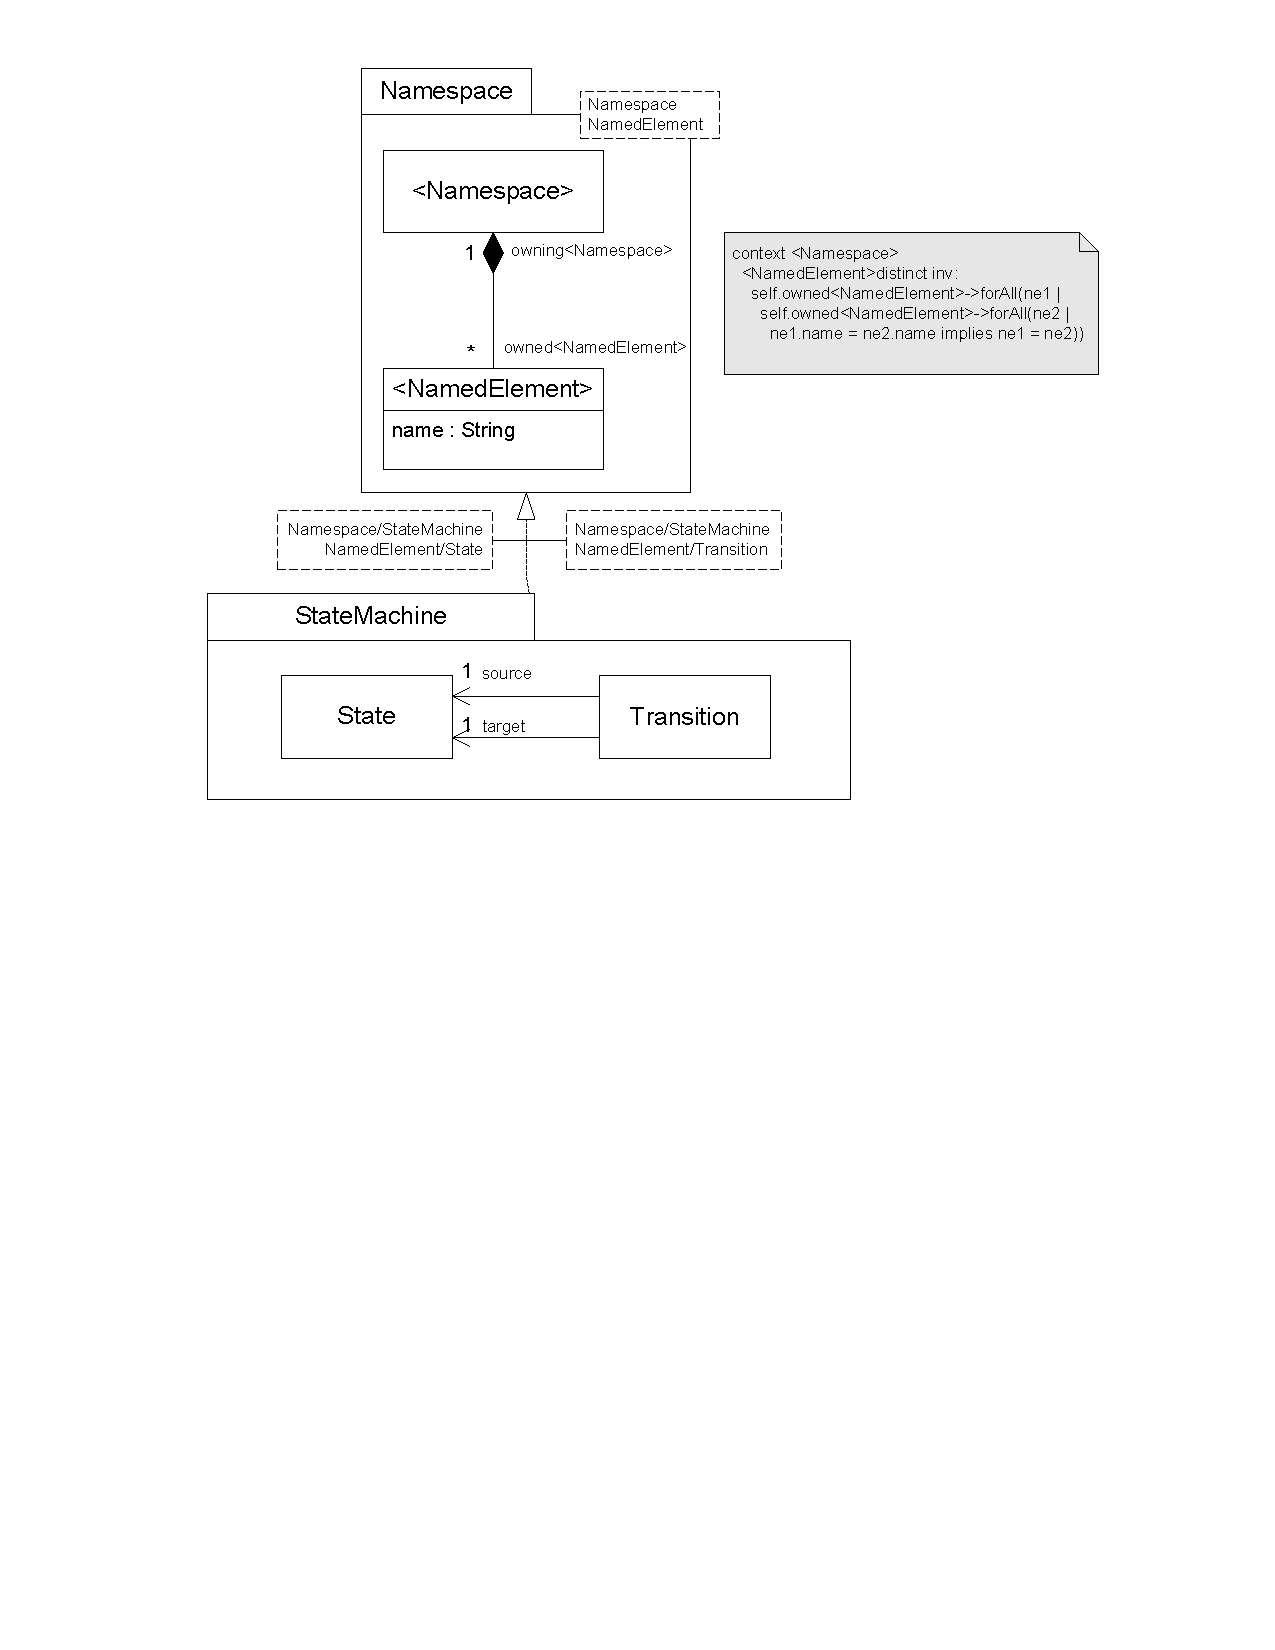
\includegraphics[width=10cm]{XMOF/figures/templateExample}
\caption{Using a template to derive the class diagram of figure \ref{classDiagram}}
\label{templateExample}
\end{center}
\end{figure}

\section{Differences from Existing Metamodelling Languages}

The requirement to be able to construct metamodels is not a new
one, and not surprisingly a variety of languages have been proposed
as metamodelling languages. The most notable of these are UML and
the MOF (the Meta Object Fa cility). The MOF is the standard
language for capturing meta-data, and goes further than the UML in
meeting the requirements of a metamodelling language. Nevertheless,
whilst the MOF provides many of the features necessary to define
metamodels, there are a number of crucial areas in which it needs
to be extended.

\begin{itemize}
\item The MOF does not explicitly support executable metamodelling in
a platform independent way. Although it does provide OCL, this does not
support the construction of operations that change the state of a model.
An alterantive might be to use the Action semantics. This is a platform
independent language for executing models, that is currently a part of
the the UML 1.5 metamodel. There are two main problems with this language
however. It is complex and does not support many of the useful set
operations offered by OCL, such as iterate, collect and select. Secondly,
it is not currently a part of the MOF metamodel. Whilst work is ongoing
 to resolve these issues, XMOF resolves them by the minimal extension of
 OCL to result in the powerful executable expression language.
\item The MOF does not support an extensible grammar language. This is
important in being able to model new concrete syntax grammars in MOF.
\item The MOF currently is not defined fully in terms of itself. Its
semantics and syntax are stated in a form (a mixture of OCL, and
informal english) that prevents it from being completely self describing
and self supporting.
\item The MOF currently does not support a pattern based mapping language
such as the XMap language described above. Work is howwever, currently
proceeding on an extension to MOF called QVT (Queries, Views, Transformations),
which aims to define a language for doing mappings, but it is unlear at this
stage whether it will support all the capabilities of XMap in the short to
medium term.
\end{itemize}

XMOF aims to provide these extensions in the most concise and
minimal fashion necessary to support precise, semantically rich
metamodelling.


\section{Conclusions}
